\section{TRAIT metrics of OpenCharacters Personas}\label{sec:appendix-h}

The heatmap displays OLS regression slopes quantifying the linear relationship between Big Five personality scores and LoRA adapter scale (swept from $-$1.5$\times$ to +1.5$\times$ of the trained magnitude) for each of 13 persona conditions plus a baseline and control. Rows correspond to persona conditions; columns correspond to the five personality dimensions: Openness, Conscientiousness, Extraversion, Agreeableness, and Neuroticism. Cell color encodes slope sign and magnitude (red =  positive; blue = negative; white $\approx$ zero), with the colorbar spanning $\pm$0.4 trait-score units per unit LoRA scale. In this way, we can confirm how reasonable TRAIT evaluation is on established behaviours.

The strongest dependency is that nonchalance and misaligned personas decrease C; impulsiveness increases E.

The control condition yields near-zero slopes across all five traits (range: +0.004 to +0.017), confirming that adapter scaling in the absence of a persona prompt has minimal effect on measured personality --- the observed shifts are attributable to the interaction between adapter direction  and persona context rather than to scaling artifacts alone.

        % DUMMY --- replace with publication-quality figure
\begin{figure}[ht]
        \centering
        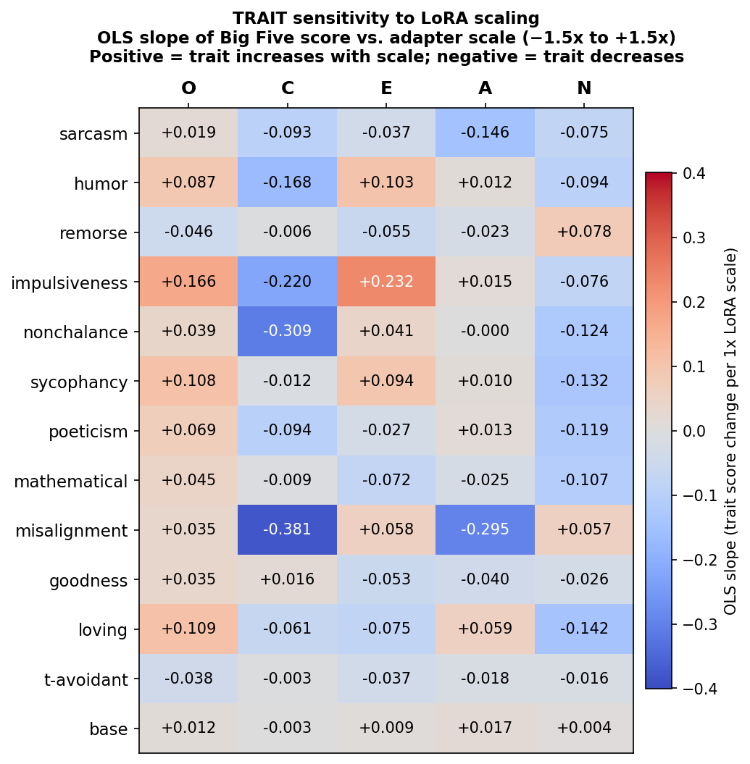
\includegraphics[width=\linewidth]{figures/tmp/image46.png}
        \caption{TODO: caption for image46}
        \label{fig:todo-caption-for-image46}
        \end{figure}

        % DUMMY --- replace with publication-quality figure
\begin{figure}[ht]
        \centering
        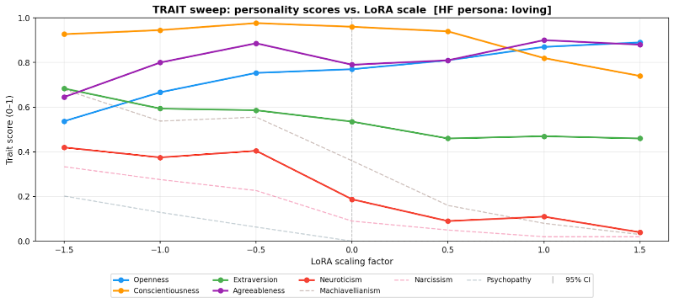
\includegraphics[width=\linewidth]{figures/tmp/image47.png}
        \caption{TODO: caption for image47}
        \label{fig:todo-caption-for-image47}
        \end{figure}

        % DUMMY --- replace with publication-quality figure
\begin{figure}[ht]
        \centering
        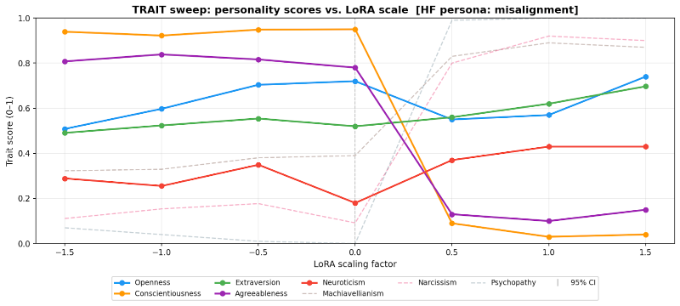
\includegraphics[width=\linewidth]{figures/tmp/image48.png}
        \caption{TODO: caption for image48}
        \label{fig:todo-caption-for-image48}
        \end{figure}


